\titre{question 1} \\ Exemple basique de fork : une variable est dupliquée du père au fils. \\
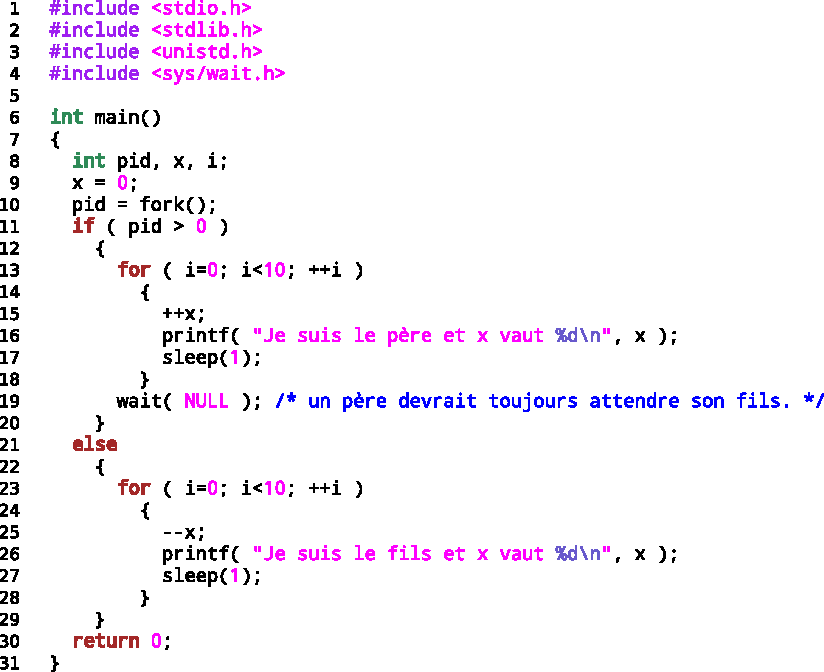
\includegraphics[width=\linewidth]{fig25.pdf}\newpage
\titre{question 2}
\begin{enumerate}
	\item Deux threads manipulent la même variable globale \\
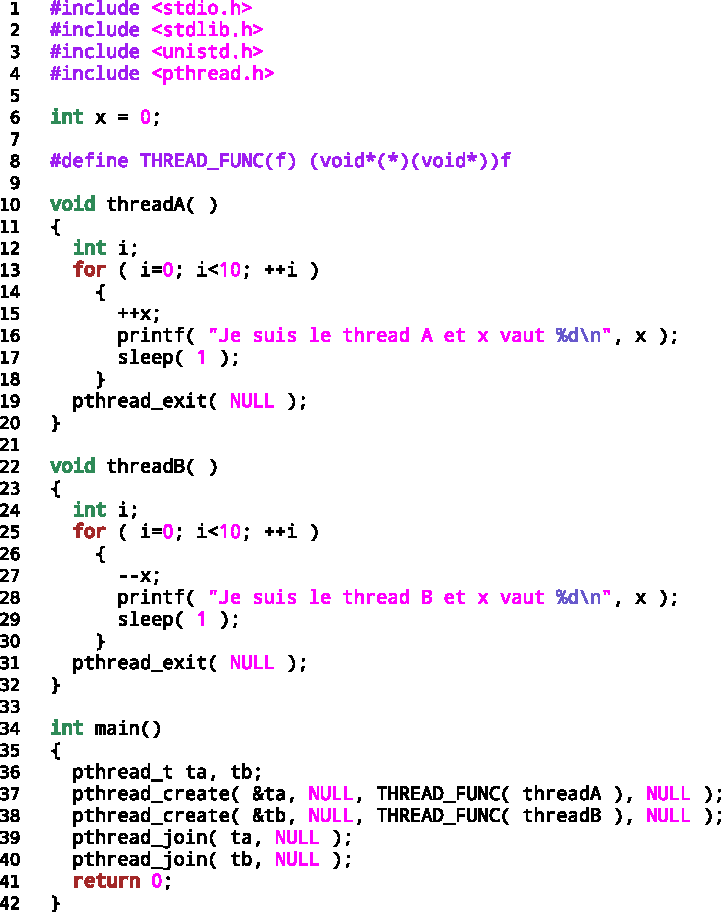
\includegraphics[width=\linewidth]{fig26.pdf}\newpage
	\item Deux threads manipulent la même variable grâce aux pointeurs \\
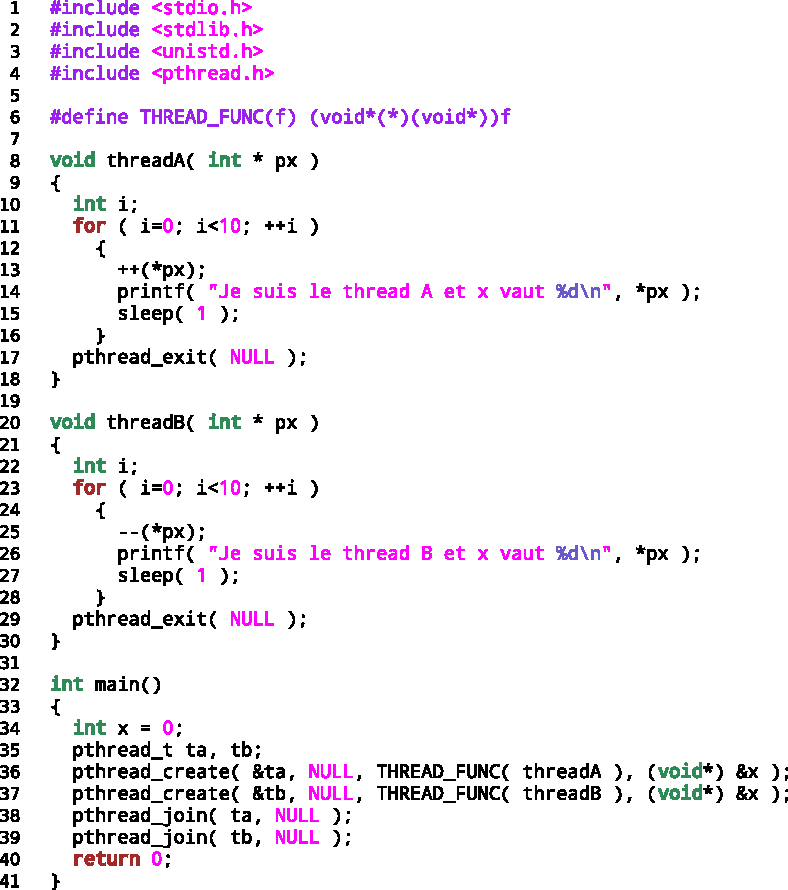
\includegraphics[width=\linewidth]{fig27.pdf}\\
\end{enumerate} \newpage
\titre{question 3}
\begin{enumerate}
	\item Deux threads décrémentent un même variable\\
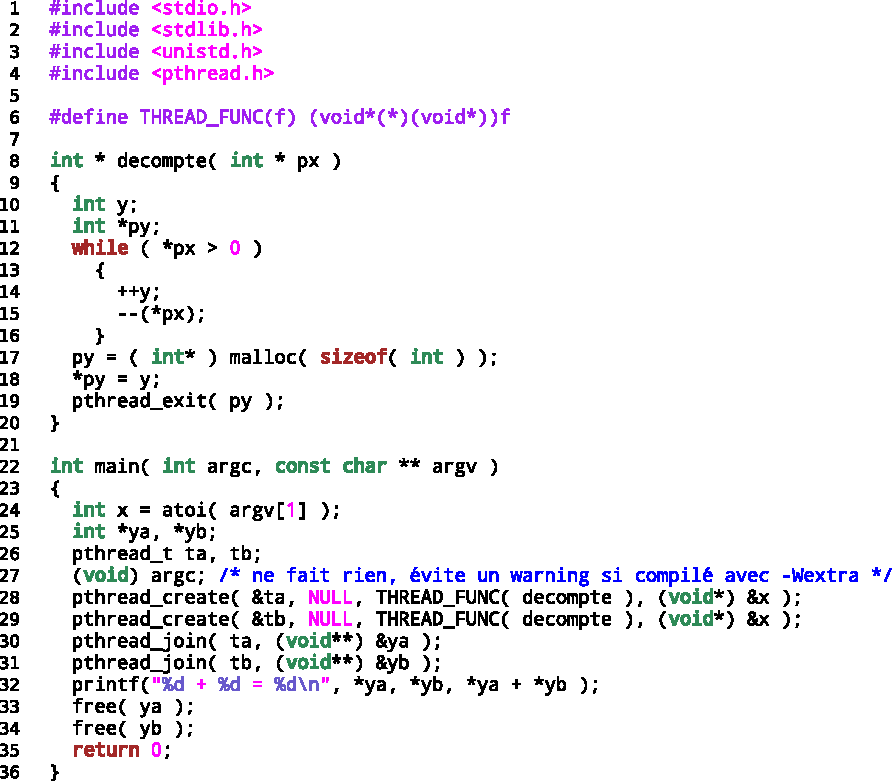
\includegraphics[width=\linewidth]{fig28.pdf}\newpage
	\item Nous essayons d'utiliser un verrou pour éviter les problèmes de concurrence (attente active)\\
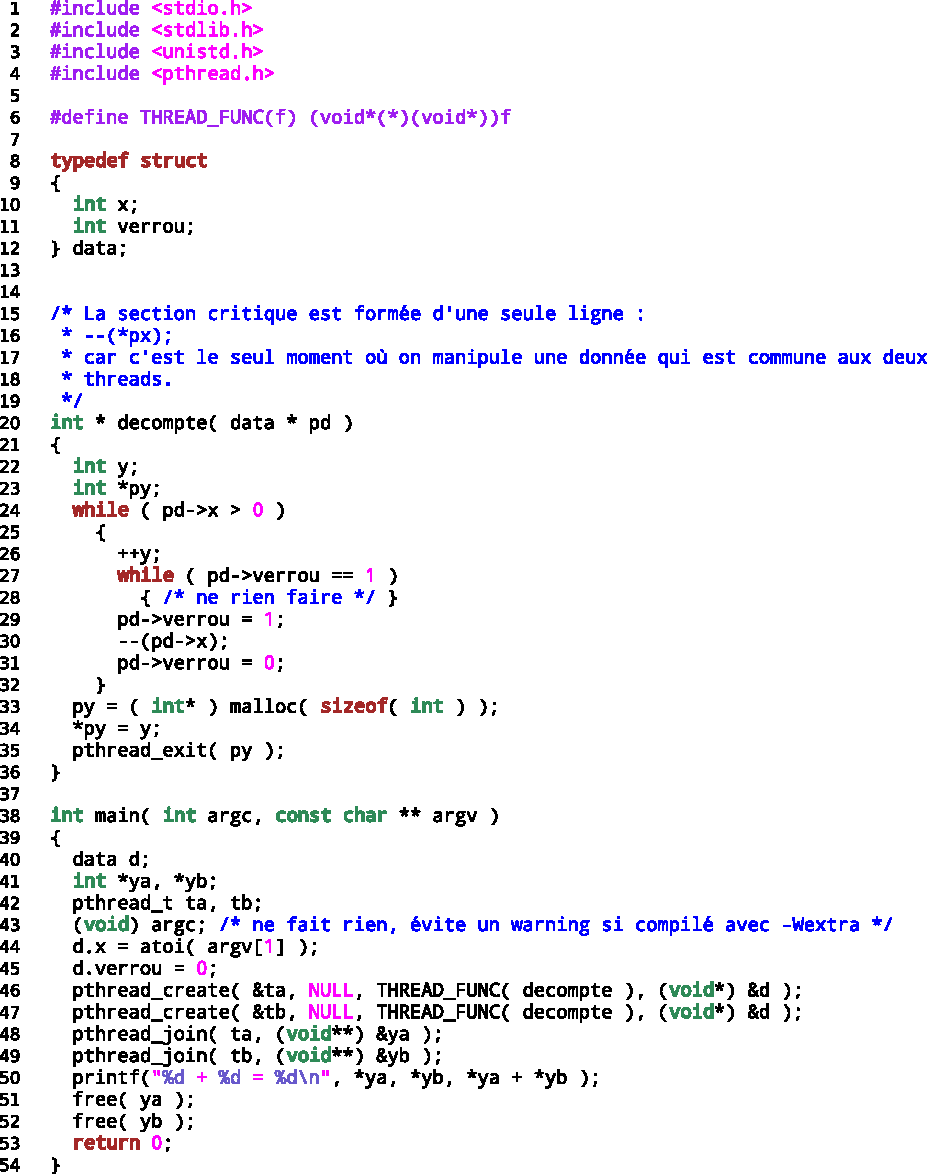
\includegraphics[width=\linewidth]{fig29.pdf}\\
\end{enumerate}
